\documentclass[12pt,fleqn]{article}\usepackage{../../common}
\begin{document}
Sonlu Öğeler  - 2. Bölüm

Üzerinden geçelim, sistem zayıf form ile ise başlar. Önceki dersin sonunda
Galerkin fikrini tanıştırdık, sürekli diferansiyel denklem yerine onu ayrıksal
temsil etmeye uğraş. Galerkin bunun için bazı deneme fonsiyonları kullanır
onlara $\phi_1,...,\phi_N$ diyelim, ayrıca test fonksiyonları da vardır
(çoğunlukla test fonksiyonları ile deneme, yani $\phi$ ve $v$ fonksiyonları
aynıdır). Bugün işleyeceğimiz bu fonksiyonların nasıl seçildiği ve hazirlik
asamasini gosterdikten sonra bunun verdigi $KU = F$ denklemin nasil
cozuldugu. $K$ nereden geliyor, $F$ nereden geliyor? $F$ bir sekilde alttaki
ikinci denklemin (oktan sonra) sag tarafindan geliyor, $K$ ise sol
tarafindan.. Detaylari simdi gorecegiz.

$$
- \frac{\ud}{\ud x} \left( c(x) \frac{\ud u}{\ud x} \right) = f(x) \to
\int _{0}^{1} c \frac{\ud u}{\ud x} \frac{\ud v}{\ud x} \ud x =
\int _{0}^{1} f(x) v(x) \ud x
$$

ki eger $u(1)=0$ ise $v(1) = 0$ (sinir sarti).

Sonlu ogeler metotunun (FEM) temeli $KU = F$. Ustteki denklemde okun sol tarafi
diferansiyel denklemimiz, sinir sartlari vs ile ``guclu formda'', oktan sonrasi
zayif form, ki onun da kendi sinir sartlari var. Sabit degiskenler guclu formdan
zayif forma geciyor, ama serbest degiskenler gecmiyor. $v$'yi $u$'dan olan ufak
sapmalar olarak gordugum icin eger $u$'yi sabitliyorsam $v$ de sabitleniyor.

Tum bunlari gorduk ama hala ayaklarimiz yere basmadi; bir cok fikirden
bahsettik, ama simdi daha gercek dunyaya baglanacagiz. Gercek dunya demek tabii
$\phi$'lerle alakali, hangi somut fonksiyonlari $\phi$ olarak sececegiz?

Acaba ornek bir $\phi$ ne olabilir? Mesela $x=2$ noktasinda tepe yapan bir
parcali lineer fonksiyon kullanabilirim,

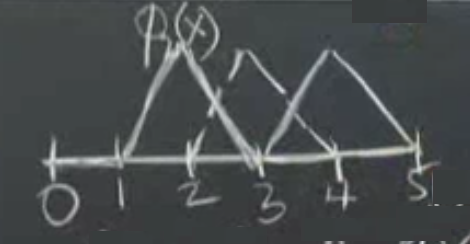
\includegraphics[width=10em]{compscieng_1_18_01.png}

Bu fonksiyona $\phi_2(x)$ diyelim, 1 ila 3 arasinda 2 uzerinde tepe yapiyor
diger yerlerde ya lineer egimi var, ya da degeri sifir. Her $\phi$ maksimum tepe
noktasi 1 olarak secilabilir. Onun sagindaki $\phi_3$ olabilir, benzer bir
fonksiyon sadece 3 degeri bazli tanimli. Buradaki ana amac sistemi basit ogeler
uzerinde insa etmek. FEM'in ana fikri budur; $\phi$ icin basit fonksiyonlar
kullan. Bu basitligin devami olarak $\phi$ ve $v$ fonksiyonlarini ayni sec.

Peki sinir noktalarinda ne olacak? Ustte serbest-sabit problemi cozecegim,
sol uc nokta serbest, sag uc nokta sabit (sinir tanimlanmis). 

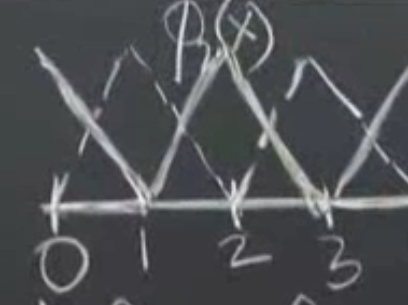
\includegraphics[width=10em]{compscieng_1_18_02.png}

Ustteki resme bakarsak, $x=0$ icin bir ``yarim sapka'' fonksiyonu tanimladim,
$\phi_0$ diyelim, ve eger diger ucgen fonksiyonlara tam sapka dersek bu da yarim
sapka. O noktada $\phi$ ve $v$'lerim kisitli degiller. Boylece elimde bes tane
deneme fonksiyonu oluyor, $\phi_0$, $\phi_1$, $\phi_2$, $\phi_3$, $\phi_4$.

Amac nedir? Yaklasik FEM cozumum $U(x)$'in ustteki basit sapka fonksiyonlarinin
bir kombinasyonu olmasini istiyorum.

$$
U(x) = U_0 \phi_0(x) + ... + U_4 \phi_4(x)
$$

$U_0,..,U_4$ degerleri skalar, tek sayi.. onlar ilk basta bilinmeyen ``agirlik''
degerleri, $\phi$'leri belli sekilde carpacaklar ve bu carpimlarin toplami
yaklasik bir $u$ olacak.

Bu kombinasyonlar neye benzerdi acaba? 

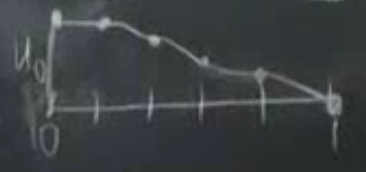
\includegraphics[width=10em]{compscieng_1_18_03.png}

Baslangictaki deger niye $u_0$? Cunku orada tum diger $\phi$ fonksiyonlari sifir
seviyesinde, hemen yandaki $\phi_1$ bile orada sifir ve maksimum $\phi$ deger 1
oldugu icin baslangic degeri $u_0$.

Bu arada Galerkin, ismini tasiyan yontemi bulurken, aklinda erismeye ugrastigi
belli bir cozum fonksiyonu vardi, ve sapka fonksiyonlarini oraya varmak icin
secmisti fakat modern FEM yaklasimlarinda, yazilimlarinda bir temel fonksiyonu
ilk bastan seceriz, problem hakkinda bir sey bilmesek bile. Sapka fonksiyonlari
bu fonksiyonlardan biridir.

Sonlu ogeler temel fonksiyonlari dugum noktalariyla baglantilidir, bu baglamda
sonlu farklilikler (finite differences) metotuna benzer (tabii FD ile esit
aralikla bolmek gerekir, FEM ile bu zorunluluk yok), ogeler dugum noktalarina
oturtuluyor. FEM ile sapka fonksiyonu ozelinde her dugum noktasindaki $u$
degerinin o noktadaki agirlik degeri ile ayni olmasini zorlamis oluyoruz; mesela
1 dugumundeki deger nedir? $u_1$! Cunku orada diger tum sapka fonksiyonlari
sifirdir, sadece $\phi_1$ degeri 1, toplanan tum terimler yokoluyor geriye
sadece $u_1 \phi_1 = u_1$ kaliyor.

FD benzerligi hakkinda, $KU=F$'i olusturdugumuzda onun bir FD denklemine oldukca
benzedigini gorecegiz, arada yapisal farklar var tabii, FD ile ayriksal
denklemleri biz tanimliyoruz, FEM ile sadece baz ogeleri seciyoruz denklemin
ne oldugunu Galerkin yontemi bize soyluyor.














[devam edecek]

\end{document}



